\documentclass[11pt]{book}
\usepackage{gvv-book}
\usepackage{gvv}
\usepackage[sectionbib,authoryear]{natbib}
\setcounter{secnumdepth}{3}
\setcounter{tocdepth}{2}
\makeindex

\begin{document}
\frontmatter
\tableofcontents
\setcounter{page}{1}
\mainmatter
\chapter{Triangle}
Consider a triangle with vertices
\begin{align}
\label{eq:tri-pts}
\vec{A}=\myvec{-3 \\ -5},\,
\vec{B}=\myvec{3\\-5},\,
	\vec{c}=\myvec{-4\\-3},\,
\end{align}

\section{Vectors}
\section{Median}
\section{Altitude}
\section{Perpendicular Bisector}

\begin{enumerate}[label=\thesection.\arabic*.,ref=\thesection.\theenumi]
\numberwithin{equation}{enumi}

%Question 1.4.1:
\item The equation of the perpendicular bisector of $BC$ is
\begin{align}
\label{eq:tri-perp-bisect}
\brak{\vec{x}-\frac{\vec{B}+\vec{C}}{2}}\brak{\vec{B}-\vec{C}} = 0
\end{align}
Substitute numerical values and find the equations of the perpendicular bisectors of $AB, BC$ and $CA$.
\\	\solution
\begin{enumerate}
    \item $\vec{BC}$: given equation for the perpendicular bisector of $\vec{BC}$:
\begin{align}
    \brak{\vec{x}-\frac{\vec{B}+\vec{C}}{2}}\brak{\vec{B}-\vec{C}} = 0
\end{align}
On substituting the values,
\begin{align}
    \vec{\frac{\vec{B}+\vec{C}}{2}} &= \myvec{\frac{-1}{2} \\ -4} \\
\vec{B}-\vec{C} &= \myvec{7 \\ -2} \\
\end{align}
solving using matrix multiplication
\begin{align}
\brak{\vec{B}-\vec{C}}^{\top}\brak{\frac{\vec{B}+\vec{C}}{2}}&=0 \\
\brak{\vec{B}-\vec{C}}^{\top} &= \myvec{7 & -2} \\
\brak{\vec{B}-\vec{C}}^{\top}\brak{\frac{\vec{B}+\vec{C}}{2}}&=\myvec{7 & -2}\myvec{\frac{-1}{2} \\ -4}\\
&= \frac{9}{2}
\end{align}
Therefore perpendicular bisector of $\vec{BC}$ is
\begin{align}
    \myvec{7 & -2}\vec{x}&= \frac{9}{2}
\end{align}

  \item $\vec{AB}$: similarly the equation for the perpendicular bisector of $\vec{AB}$:
\begin{align}
    \brak{\vec{x}-\frac{\vec{A}+\vec{B}}{2}}\brak{\vec{A}-\vec{B}} = 0
\end{align}
On substituting the values,
\begin{align}
    \vec{\frac{\vec{A}+\vec{B}}{2}} &= \myvec{0 \\ -5} \\
\vec{A}-\vec{B} &= \myvec{-6 \\ 0} \\
\end{align}
solving using matrix multiplication
\begin{align}
\brak{\vec{A}-\vec{B}}^{\top}\brak{\frac{\vec{A}+\vec{B}}{2}}&=0 \\
\brak{\vec{A}-\vec{B}}^{\top} &= \myvec{-6 & 0} \\
\brak{\vec{A}-\vec{B}}^{\top}\brak{\frac{\vec{A}+\vec{B}}{2}}&=\myvec{-6 & 0}\myvec{0 \\ -5}\\
&= 0
\end{align}
Therefore perpendicular bisector of $\vec{AB}$ is
\begin{align}
    \myvec{-6 & 0}\vec{x}&= 0
\end{align}

  \item $\vec{CA}$: similarly the equation for the perpendicular bisector of $\vec{CA}$:
\begin{align}
    \brak{\vec{x}-\frac{\vec{C}+\vec{A}}{2}}\brak{\vec{C}-\vec{A}} = 0
\end{align}
On substituting the values,
\begin{align}
    \vec{\frac{\vec{C}+\vec{A}}{2}} &= \myvec{\frac{-7}{2} \\ -4} \\
\vec{C}-\vec{A} &= \myvec{-1 \\ 2} \\
\end{align}
solving using matrix multiplication
\begin{align}
\brak{\vec{C}-\vec{A}}^{\top}\brak{\frac{\vec{C}+\vec{A}}{2}}&=0 \\
\brak{\vec{C}-\vec{A}}^{\top} &= \myvec{-1 & 2} \\
\brak{\vec{C}-\vec{A}}^{\top}\brak{\frac{\vec{C}+\vec{A}}{2}}&=\myvec{-1 & 2}\myvec{\frac{-7}{2} \\ -4}\\
&= \frac{-9}{2}
\end{align}
Therefore perpendicular bisector of $\vec{BC}$ is
\begin{align}
    \myvec{-1 & 2}\vec{x}&= \frac{-9}{2}
\end{align}
\end{enumerate}

\begin{figure}[H]
\centering
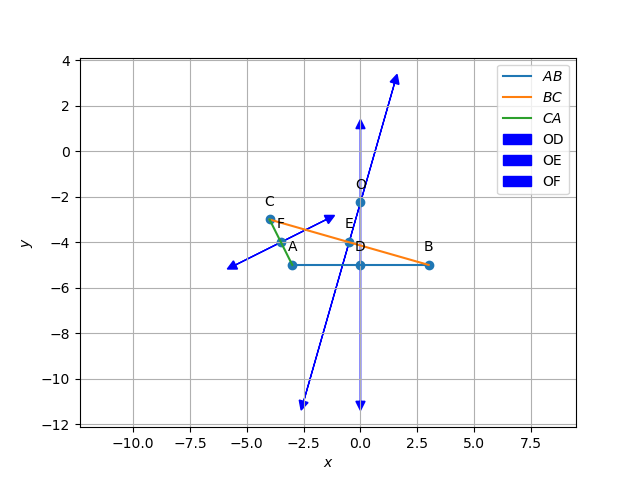
\includegraphics[width=\columnwidth]{figs/perp_bisect1.png}
\caption{Plot of the perpendicular bisectors}
\label{fig:figure1}
\end{figure}


%Question 1.4.2:
\item Find the intersection $\vec{O}$ of the perpendicular bisectors of $AB$ and $AC$.
 \\
\solution \\
\begin{figure}[H]
\centering
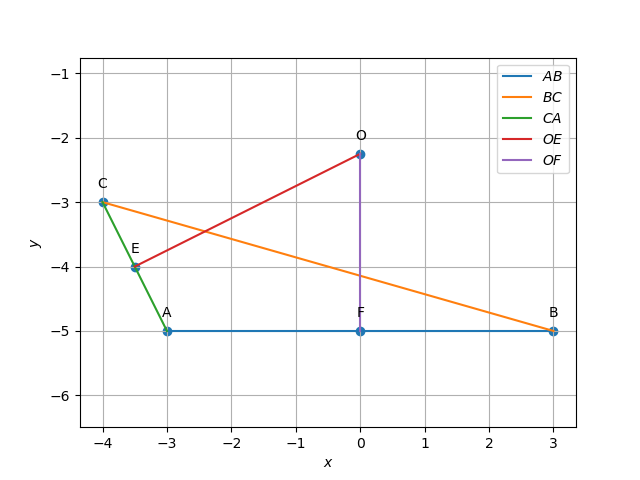
\includegraphics[width=\columnwidth]{figs/perp_bisect2.png}
\caption{$\vec{O}-\vec{E}$ and $\vec{O}-\vec{F}$ are perpendicular bisectors of $\vec{A}-\vec{C}$ and $\vec{A}-\vec{B}$ respectively}
\label{fig:Figure_2}
\end{figure}

Given,
\begin{align}
\vec{A}=\myvec{-3 \\ -5},\,
\vec{B}=\myvec{3\\-5},\,
	\vec{c}=\myvec{-4\\-3},\,
\end{align}

Vector equation of perpendicular bisector of $\vec{A}-\vec{B}$ is
\begin{align}
 (\vec{A}-\vec{B})^\top  \brak{ \vec{x} - \frac{\vec{A}+\vec{B}}{2}} = 0
\end{align}
where,
\begin{align}
\vec{A}+\vec{B}&=\myvec{-3\\-5}+\myvec{3\\-5}\\
&=\myvec{0\\-10}\\
\vec{A}-\vec{B} &= \myvec{-3\\-5}-\myvec{3\\-5}\\
&=\myvec{-6\\0}\\
\implies (\vec{A}-\vec{B})^\top &= \myvec{-6&0}
\end{align}
$\therefore $ The vector equation of $\vec{O}-\vec{F}$ is
\begin{align}
\myvec{-6&0} \brak{ \vec{x}-\myvec{0\\-5} }&=0\\
\implies \myvec{-6&0}\vec{x}&=\myvec{-6&0}\myvec{0\\-5}
\end{align}
Performing matrix multiplication yields
\begin{align}
\myvec{-6&0}\vec{x}&=0
\end{align}\\

Vector equation of perpendicular bisector of $\vec{A}-\vec{C}$ is
\begin{align}
(\vec{A}-\vec{C})^\top\brak{ \vec{x} - \frac{\vec{A}+\vec{C}}{2}} = 0
\end{align}
where,
\begin{align}
\vec{A}+\vec{C}&=\myvec{-3\\-5}+\myvec{-4\\-3}\\
&=\myvec{-7\\-8}\\
\vec{A}-\vec{C} &= \myvec{-3\\-5}-\myvec{-4\\-3}\\
&=\myvec{1\\-2}\\
\implies (\vec{A}-\vec{C})^\top &= \myvec{1&-2}
\end{align}
$\therefore $ The vector equation of $\vec{O}-\vec{E}$ is
\begin{align}
\myvec{1&-2}\brak{ \vec{x}-\frac{1}{2}\myvec{-7\\-8}}&=0\\
\implies \myvec{1&-2}\vec{x}&=\frac{1}{2}\myvec{1&-2}\myvec{-7\\-8}
\end{align}
Performing matrix multiplication yields
\begin{align}
\myvec{1&-2}\vec{x}&=\frac{9}{2}
\end{align}

Thus,
\begin{align}
\myvec{-6&0&0\\1&-2&\frac{9}{2}} &\xleftrightarrow[]{R_1 \leftarrow \frac{-1}{6} R_1} \myvec{1&0&0\\1&-2&\frac{9}{2}}\\
\myvec{1&0&0\\1&-2&\frac{9}{2}} &\xleftrightarrow[]{R_2\leftarrow R_2 - R_1}
\myvec{1&0& 0\\0&-2&\frac{-9}{2}}\\
\myvec{1&0& 0\\0&-2&\frac{-9}{2}} &\xleftrightarrow[]{R_2 \leftarrow \frac{-1}{2}R_2} \myvec{1&0&0 \\0&1&\frac{-9}{4}}\\
\therefore \myvec{1&0\\0&1}\vec{x} &= \myvec{0\\\frac{-9}{4}}\\
\implies \vec{x}&=\myvec{0\\\frac{-9}{4}}
\end{align}
Therefore, the point of intersection of perpendicular bisectors of $\vec{A}-\vec{B}$ and $\vec{A}-\vec{C}$ is $\vec{O} = \myvec{0\\ \frac{-9}{4}}$

 %Question 1.4.3:
\item Verify that $\vec{O}$ satisfies
			\eqref{eq:tri-perp-bisect}.
$\vec{O}$ is known as the circumcentre.\\
 \solution
 From the previous question we get,
 \begin{align}
\vec{O}&=\myvec{0\\ \frac{-9}{4}} \\
\brak{\vec{x}-\frac{\vec{B}+\vec{C}}{2}}\brak{\vec{B}-\vec{C}} &= 0
\end{align}
when substituted in the above equation,
\begin{align}
	&=\brak{\vec{O}-\frac{\vec{B}+\vec{C}}{2}}.\brak{\vec{B}-\vec{C}}\\
	&=\brak{\myvec{0\\ \frac{-9}{4}}- \frac{1}{2}\myvec{-2\\-8}}^{\top} \myvec{7\\-2}\\
	&=\myvec{\frac{1}{2}& \frac{7}{4}}\myvec{7\\-2}\\
	&=0
\end{align}
It is hence proved that $\vec{O}$ satisfies the equation \eqref{eq:tri-perp-bisect}
\begin{figure}[H]
\centering
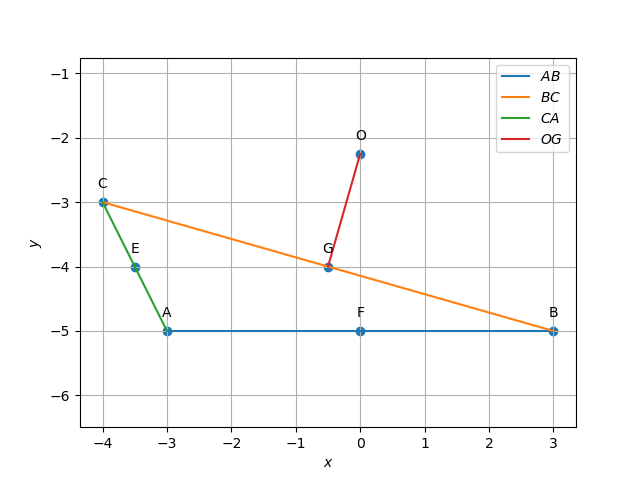
\includegraphics[width=\columnwidth]{figs/perp_bisect3.png}
\caption{Circumcenter plotted using python}
\label{fig:Circumcenter to BC}
\end{figure}

 %Question 1.4.4:  
\item Verify that 
\begin{align}
OA = OB = OC 
\end{align} 
\solution
Given \begin{align}
\vec{A} &= \myvec{-3\\-5}\\
\vec{B} &= \myvec{3\\-5}\\
\vec{C} &= \myvec{-4\\-3}
\end{align}
From problem-1.4.2 :
\begin{align}
O &= \myvec{0 \\ \frac{-9}{4}}\\
 &= \myvec{0\\ -2.25}
\end{align}
\begin{enumerate}
\item 
\begin{align}
OA &= \sqrt{(\vec{O}-\vec{A})^{\top}(\vec{O}-\vec{A})}\\
&= \sqrt{\myvec{3 & \frac{11}{4}} \myvec{3\\ \frac{11}{4}}}\\
 &= \sqrt{\frac{265}{16}}\\
 &= \frac{\sqrt{265}}{4}
\end{align}
\item 
\begin{align}
OB &= \sqrt{(\vec{O}-\vec{B})^{\top}(\vec{O}-\vec{B})}\\
 &= \sqrt{\myvec{-3 & \frac{11}{4}} \myvec{-3\\ \frac{11}{4}}}\\
 &= \sqrt{\frac{265}{16}}\\
 &= \frac{\sqrt{265}}{4}
\end{align}
\item 
\begin{align}
OC &= \sqrt{(\vec{O}-\vec{C})^{\top}(\vec{O}-\vec{C})}\\
 &= \sqrt{\myvec{4 & \frac{3}{4}}  \myvec{4\\ \frac{3}{4}}}\\
 &= \sqrt{\frac{265}{16}}\\
 &= \frac{\sqrt{265}}{4}
\end{align}
\end{enumerate}
From above, 
\begin{align}
OA = OB = OC
\end{align}
Hence verified.

%Question 1.4.5:
\item Draw the circle with centre at $\vec{O}$ and radius 
\begin{align}
R = OA
\end{align}
This is known as the {\em circumradius}. \\
\solution
Given
\begin{align}
\vec{A} &= \myvec{-3\\-5}\\
\vec{B} &= \myvec{3\\-5}\\
\vec{C} &= \myvec{-4\\-3}
\end{align}
From Q1.4.2, the circumcentre is
\begin{align}
\vec{O} = \myvec{0\\ \frac{-9}{4}}
\end{align}
Now we will calculate the radius,
\begin{align}
      R &= OA\\
        &= \norm{\vec{A} - \vec{O}}\\
        &= \norm{\myvec{-3\\-5} - \myvec{0\\ \frac{-9}{4}}}\\
        &= \norm{\myvec{-3\\ \frac{-11}{4}}}\\
        &=\sqrt{\myvec{-3 & \frac{-11}{4}}\myvec{-3 \\ \frac{-11}{4}}} \\
        &= \frac{\sqrt{265}}{4}
\end{align}
see \figref{fig:circumcircle with centre O}
\begin{figure}[H]
\centering
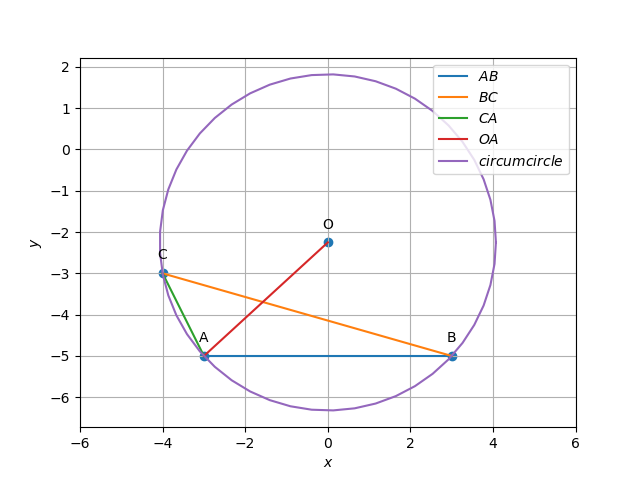
\includegraphics[width=\columnwidth]{figs/perp_bisect5.png}
\caption{circumcircle of Triangle ABC with centre O}
\label{fig:circumcircle with centre O}	
\end{figure}

 %Question 1.4.6:
\item Verify that 
\begin{align}
\angle BOC = 2\angle BAC.
\end{align}\\
 \solution
\begin{enumerate}
\item To find  the value of $\angle{BOC}$ :
\begin{align}
\vec{B}-\vec{O}
          &=\myvec{3\\\frac{-11}{4}} \\
\vec{C}-\vec{O}
         & =\myvec{-4\\\frac{-3}{4}}
	  \\
\implies \brak{\vec{B}-\vec{O}}^{\top}\brak{\vec{C}-\vec{O}}&=\frac{-159}{16}\\
	\implies \norm{\vec{B}-\vec{O}}&= \frac{\sqrt{265}}{4} \\
	\norm{\vec{C}-\vec{O}} &= \frac{\sqrt{265}}{4}
\end{align}
Thus,
\begin{align}
\cos{BOC}&=\frac{\brak{\vec{B}-\vec{O}}^{\top}\brak{\vec{C}-\vec{O}}}{\norm{\vec{B}-\vec{O}}\norm{\vec{C}-\vec{O}}}
=\frac{-159}{265}\\
\implies\angle{BOC}&=\cos^{-1}\brak{\frac{-159}{265}}
\\
	&=116.5650\degree
\end{align}
Taking the reflex of above angle we get 
\begin{align}
    \angle{BOC}&=360\degree-116.5650\degree \\
    &= 233.130\degree
\end{align}
	\item To find  the value of $\angle{BAC}$ :
\begin{align}
\vec{B}-\vec{A}&=\myvec{6\\0} \\
\vec{C}-\vec{A}&=\myvec{-1\\2}
\\
\implies \brak{\vec{B}-\vec{A}}^{\top}\brak{\vec{C}-\vec{A}}&=-6
\\
	\norm{\vec{B}-\vec{A}}&= \sqrt{36}= 6
	\norm{\vec{C}-\vec{A}}= \sqrt{5}
\end{align}
Thus,
\begin{align}
\cos{BAC}&=\frac{\brak{\vec{B}-\vec{A}}^{\top}\brak{\vec{C}-\vec{A}}}{\norm{\vec{B}-\vec{A}}\norm{\vec{C}-\vec{A}}}
=\frac{-1}{\sqrt{5}}\\
\implies\angle{BAC}&=\cos^{-1}\brak{\frac{-1}{\sqrt{5}}}\\
&=116.565\degree \label{eq:2}  \\
2\times\angle{BAC} &= 233.130
\end{align}
From \eqref{eq:2} and \eqref{eq:1},
\begin{align}
2\times\angle{BAC}
= \angle{BOC}
\end{align}
Hence Verified
\end{enumerate}

  %Question 1.4.7:
\item Let 
\begin{align}
\vec{P} = \myvec{\cos \theta & -\sin \theta \\ \sin \theta & \cos \theta}
\end{align}
Find $\theta$ if 
\begin{align}
\vec{C}-\vec{O}=\vec{P}\brak{\vec{A}-\vec{O}}
\end{align}
\solution
\begin{align}
    \vec{C}-\vec{O}
          & =\myvec{-4\\\frac{-3}{4}}\\
\vec{A}-\vec{O}
         & =\myvec{-3\\\frac{-11}{4}}
	  \\
\vec{P} &= \myvec{\cos \theta & -\sin \theta \\ \sin \theta & \cos \theta} \\
   \vec{C}-\vec{O}&=\vec{P}\brak{\vec{A}-\vec{O}} \label{eq:1.4.7.6}
\end{align}
 Now from \eqref{eq:1.4.7.6}
 \begin{align}
 \myvec{-4\\\frac{-3}{4}}&= \myvec{\cos \theta & -\sin \theta \\ \sin \theta & \cos \theta} \myvec{-3\\\frac{-11}{4}}    
 \end{align}
solving using matrix multiplication,we get
\begin{align}
    \myvec{-4\\\frac{-3}{4}}&=\myvec{ -3\cos\theta + \frac{11}{4}\sin\theta \\ -3\sin\theta + \frac{-11}{4}\cos\theta}
\end{align}
Comparing on Both sides ,we get
\begin{align}
     -3\cos\theta + \frac{11}{4}\sin\theta &= -4   \label{eq:1.4.7.9}\\
 -3\sin\theta + \frac{-11}{4}\cos\theta &= \frac{-3}{4} \label{eq:1.4.7.10}
\end{align}
On solving equations \eqref{eq:1.4.7.9}  and \eqref{eq:1.4.7.10}
\begin{align}
    \cos\theta&= \frac{45}{53} \\
    \sin\theta&= \frac{-28}{53} \\
    \theta &=\cos^{-1}\frac{45}{53} \\
            &= 31.8907 \\
            \therefore \theta = 31.8907
\end{align}
\end{enumerate}
\end{document}
